\chapter{Ένα κεφάλαιο με παραδείγματα}\label{chap:sample-chapter}
\begin{refsection}
\chapterauthor{Γιώργος Παπανικολάου}[Γιώργος Παπανικολάου \\ Χαροκόπειο Πανεπιστήμιο]
\begin{summary}{Περίληψη}
To κεφάλαιο αυτό είναι μια συρραφή από διάφορα παραδείγματα συγγραφής σε \XeLaTeX\ και δημιουργήθηκε προκειμένου να αναδείξει τις δυνατότητες του τύπου εγγράφου \emph{Kallipostd}.  Έχουν χρησιμοποιηθεί αποσπάσματα του κεφαλαίου 11 της βιβλιογραφικής αναφοράς \cite{pap}...\\
Ο νόμος των Hardy-Weinberg μάς επιτρέπει να προβλέψουμε τις συχνότητες των γονότυπων στα άτομα της επόμενης γενιάς, όταν γνωρίζουμε τις συχνότητες των αλληλόμορφων σε έναν γενετικό τόπο. Eφόσον ισχύουν οι παραδοχές στις οποίες στηρίζεται το μαθηματικό μοντέλο του νόμου, τόσο οι συχνότητες των αλληλόμορφων όσο και οι συχνότητες των γονότυπων θα παραμένουν σταθερές στις επόμενες γενεές. \\
\textbf{Προαπαιτούμενη γνώση}:Κατανόηση της ισορροπίας Hardy-Weinberg, βασικών αρχών της θεωρίας των πιθανοτήτων και του ελέγχου υποθέσεων με τη δοκιμασία $X^2$. Προηγούμενη μελέτη των βασικών αρχών θεωρίας της πληθυσμιακής γενετικής του ανθρώπου.
\end{summary}

\section{Διάφορα παραδείγματα}
\label{sec:exapmples}
\subsection{Κείμενο με βιβλιογραφικές αναφορές}
\label{subsec:text-ref}
Στο τέλος μιας διάλεξης του Reginald Punnet τον Φεβρoυάριο του 1908, ο στατιστικός Udny Yule
(1871-1951) έκανε μια ενδιαφέρουσα ερώτηση σχετικά με την κατανομή της βαραχυδακτυλίας, οι
περισσότεροι τύποι της οποίας οφείλονται σε ένα επικρατές αλληλόμορφο. Ο Yule υπέθεσε ότι
δεδομένου ότι το αλληλόμορφο είναι επικρατές, θα έπρεπε σε κάθε άνθρωπο χωρίς βραχυδακτυλία να
αντιστοιχούν τρεις περιπτώσεις με βραχυδακτυλία. Ωστόσο, κάτι τέτοιο δεν συνέβαινε στην
πραγματικότητα. Γιατί;

Μετά την ερώτηση του Yule, ο Punnet προσέτρεξε για βοήθεια στον συνάδελφό του και συμπαίκτη του
στο κρίκετ, τον μαθηματικό Godfrey Hardy (1877-1947). Ο Punnet δεν μπορούσε να ερμηνεύσει γιατί
ένα επικρατές χαρακτηριστικό δεν θα εξαπλωνόταν σταδιακά στον πληθυσμό και ένα υποτελές
αλληλόμορφο δεν θα εξαφανιζόταν. Με άλλα λόγια, δεν μπορούσε να ερμηνεύσει γιατί ένα έθνος δεν θα
γινόταν σιγά σιγά βραχυδακτυλικό. Γνωρίζοντας ότι ο Hardy ενδιαφερόταν για τα
καθαρά μαθηματικά, διατύπωσε το ερώτημα με μαθηματικούς όρους και ο Hardy το έλυσε πολύ γρήγορα,
δημοσιεύοντας την εργασία του το 1908 \cite{pmid15369635, pmid17779291}. Ο Hardy δεν μπορούσε να
φανταστεί τη θεμελιώδη επίδραση που θα είχε η συνεισφορά του στη γενετική. Ο Punnet, που
αναγνώρισε τη σημασία της, αναφερόταν σε αυτή σαν τον <<νόμο του Hardy>>. Αργότερα, διαπιστώθηκε
ότι ο γερμανός γιατρός Wilhelm Weinberg (1862-1937) είχε καταλήξει ανεξάρτητα στα ίδια
συμπεράσματα, που παρουσίασε σε μια διάλεξη το 1908. Προκειμένου να αναγνωριστεί η συνεισφορά και
των δύο επιστημόνων, ο γενετιστής Curt Stern πρότεινε η θεμελιώδης αυτή αρχή να ονομαστεί <<νόμος
των Hardy-Weinberg>> \cite{9780470464670}.
\subsection{Κώδικας}
\label{subsec:code}
Παρακάτω βλέπετε ένα παράδειγμα συγγραφής υπολογιστικού κώδικα με το πακέτο \texttt{listing}:
\begin{lstlisting}[language=R]
> library(HardyWeinberg)
> setwd("diadromi_pros_ton_katalogo_ergasias")
> B=matrix(c(16,86,23),nrow=1,ncol=3,byrow=TRUE)
> colnames(B)<-c("AA","AG","GG")
> B
	AA	AG	GG
[1,]	16	86	23
> svg(filename="kuru1.svg")
> HWTernaryPlot(B,region=1,vertex.cex=2,curvecols=c("green","red"),
signifcolour=TRUE)
> dev.off()
\end{lstlisting}

Εδώ φαίνεται το ίδιο παράδειγμα με τη χρήση του περιβάλλοντος \texttt{verbatim}:
\begin{verbatim}
> library(HardyWeinberg)
> setwd("diadromi_pros_ton_katalogo_ergasias")
> B=matrix(c(16,86,23),nrow=1,ncol=3,byrow=TRUE)
> colnames(B)<-c("AA","AG","GG")
> B
	AA	AG	GG
[1,]	16	86	23
> svg(filename="kuru1.svg")
> HWTernaryPlot(B,region=1,vertex.cex=2,curvecols=c("green","red"),
signifcolour=TRUE)
> dev.off()
\end{verbatim}

\subsection{Εικόνες και σχήματα}
Προτιμάτε να τοποθετείτε τις εικόνες-σχήματα στο άνω μέρος της σελίδας. Στην περιγραφή της λεζάντας
σημειώστε την προέλευση της εικόνας ή του σχήματος.
\begin{figure}[t]
\renewcommand{\figurename}{Εικόνα}
\centering
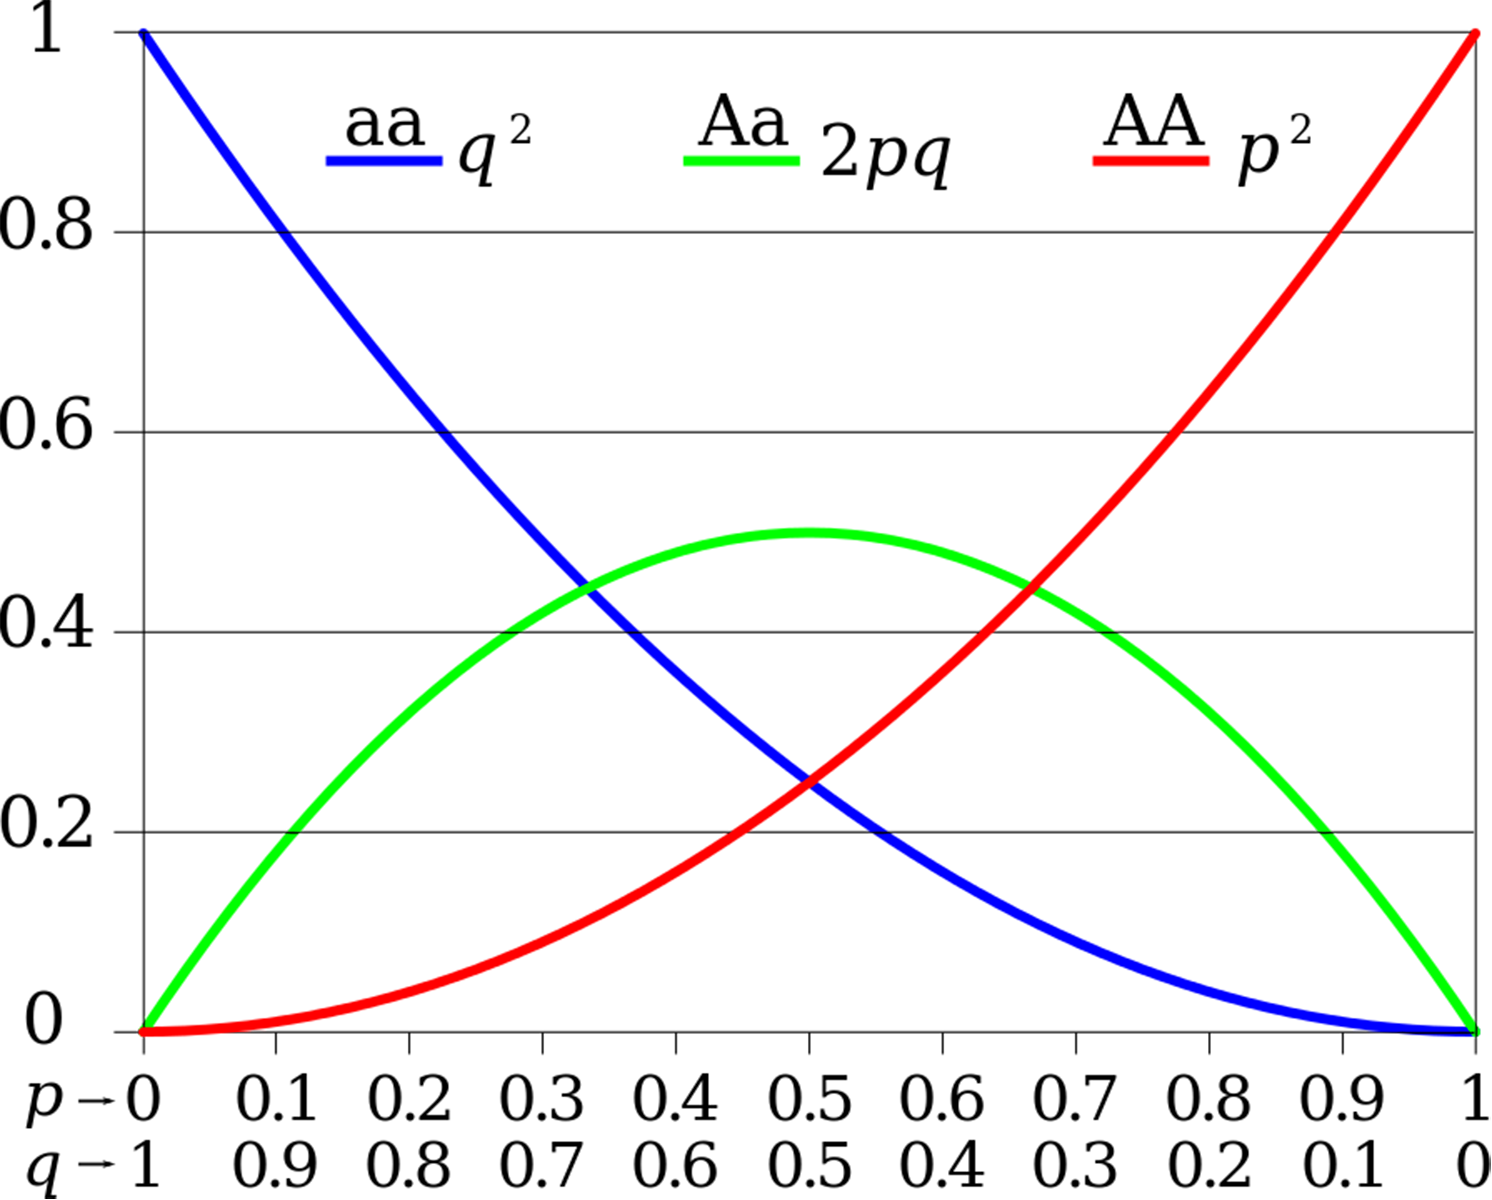
\includegraphics[width=0.4\textwidth]{images/img_7_1.png}
\caption[Αναπαράσταση ισορροπίας Hardy-Weinberg]{Αναμενόμενες συχνότητες της ισορροπίας Hardy-Weinberg για έναν γενετικό τόπο με δύο αλληλόμορφα (\href {https://commons.wikimedia.org/wiki/File:Hardy-Weinberg.svg\#/media/File:Hardy-Weinberg.svg}{πηγή: "Hardy-Weinberg" από Wikimedia Commons}).}
\label{figure:img_7_1}
\end{figure}

Ένα παράδειγμα τοποθέτησης εικόνων δίπλα-δίπλα με ενιαία λεζάντα από κάτω (εικόνα \ref{fig:double}):
\begin{figure}
\renewcommand{\figurename}{Εικόνα}
\centering
\begin{subfigure}{.5\textwidth}
  \centering
  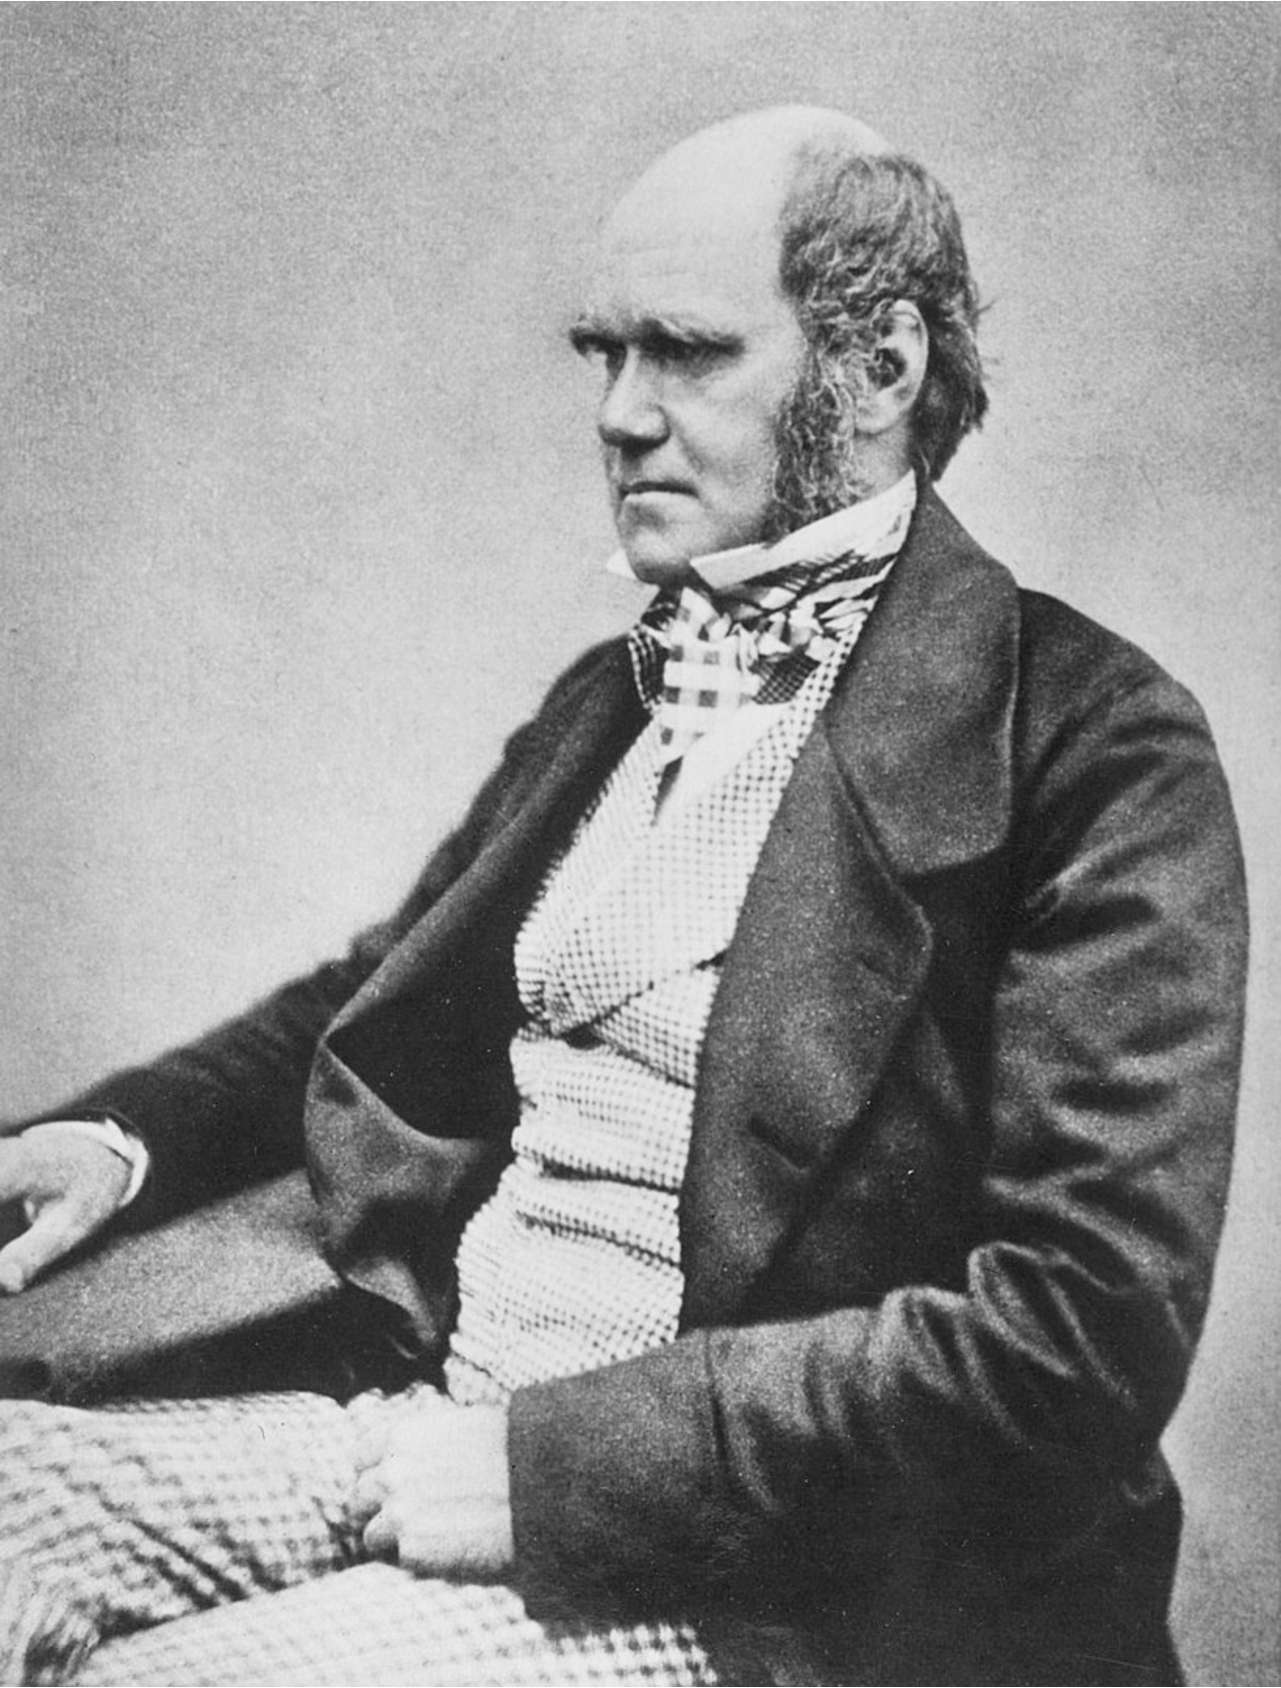
\includegraphics[width=.7\linewidth]{images/darwin.pdf}
  \caption{Charles Robert Darwin (1809-1882)}
  \label{fig:sub1}
\end{subfigure}%
\begin{subfigure}{.5\textwidth}
  \centering
  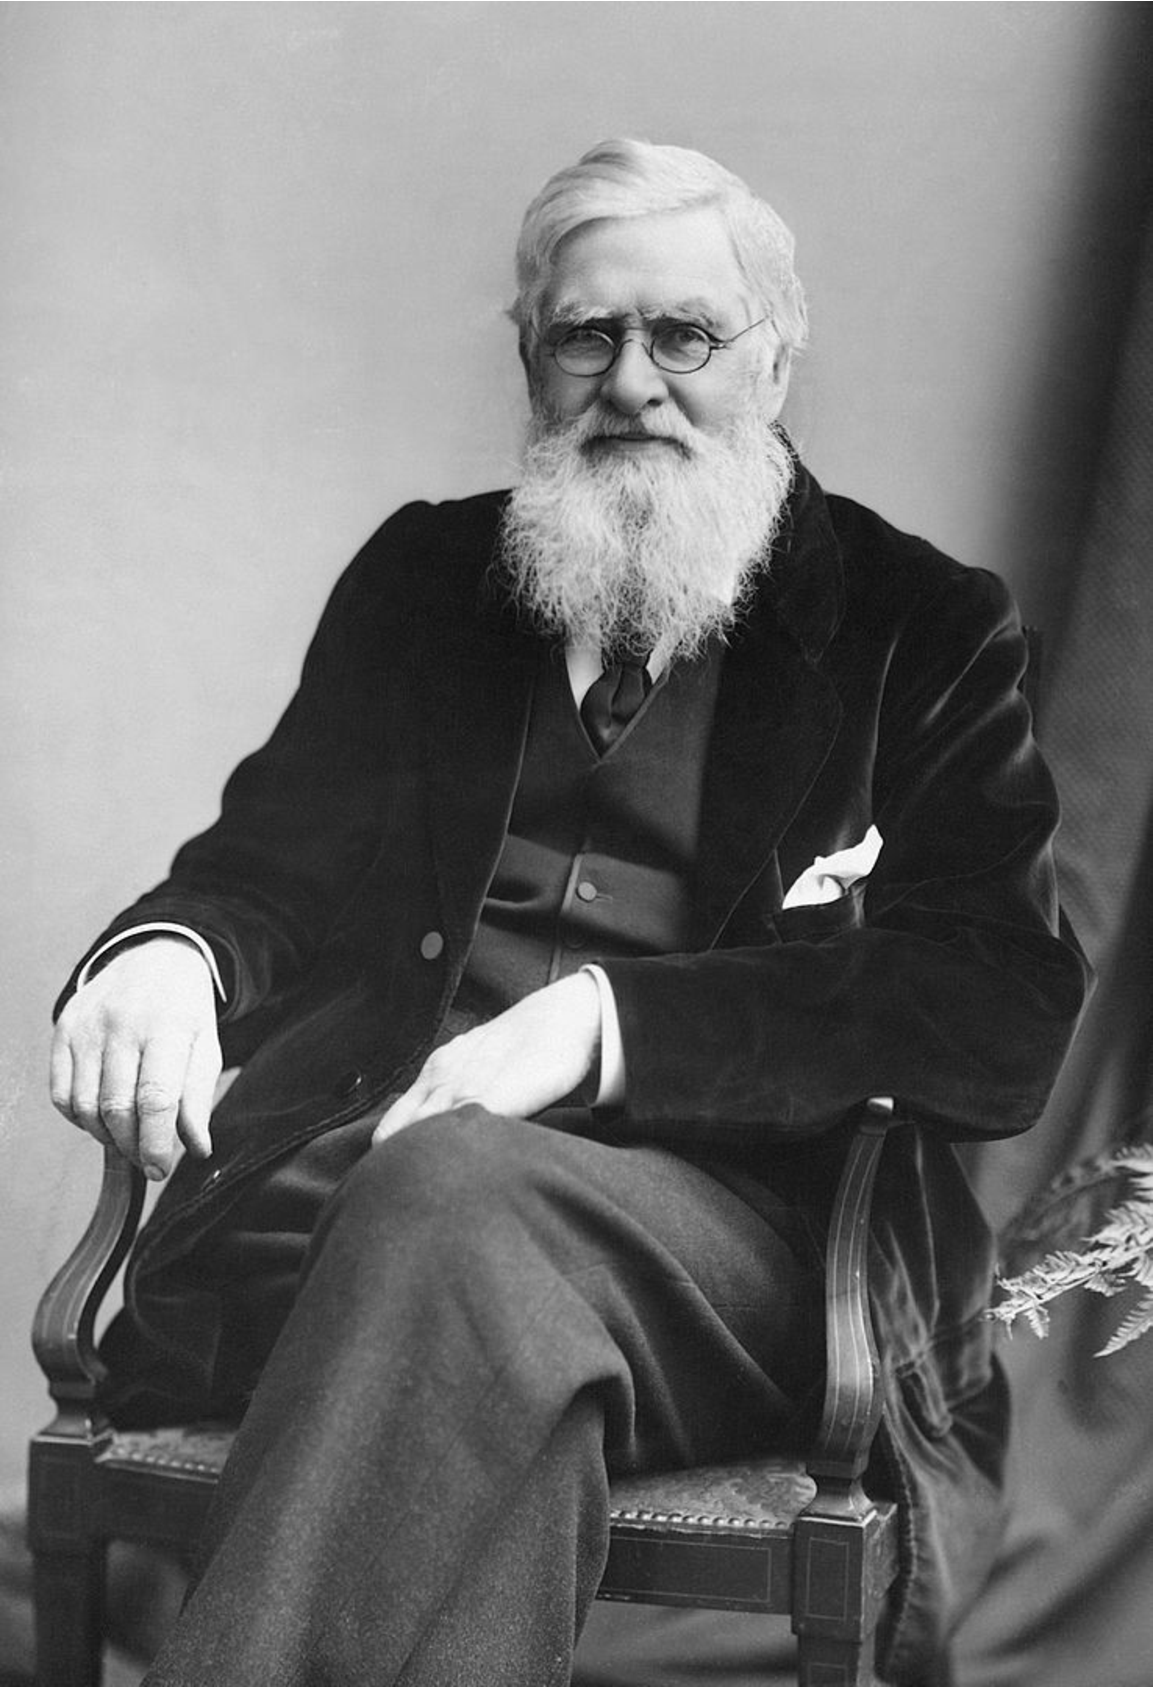
\includegraphics[width=.63\linewidth]{images/wallace.pdf}
  \caption{Alfred Russel Wallace (1823-1913)}
  \label{fig:sub2}
\end{subfigure}
\caption[Οι θεμελιωτές της εξελικτικής θεωρίας]{Οι θεμελιωτές της εξελικτικής θεωρίας. Πηγή: (α) Messrs. Maull and Fox, 1854 \href{https://commons.wikimedia.org/wiki/File:Charles_Darwin_seated_crop.jpg}{(Wikimedia Commons)}   (β) London Stereoscopic and Photographic Company, \href{https://commons.wikimedia.org/w/index.php?curid=27755581}{(Wikimedia Commons)}. }
\label{fig:double}
\end{figure}
Στην εικόνα \ref{fig:double} έχουν χρησιμοποιηθεί τα πακέτα:
\begin{verbatim}
\usepackage{caption}
\usepackage{subcaption}
\end{verbatim}
\subsection{Μαθηματικά}
\paragraph{Χρήση του περιβάλλοντος \texttt{equation}}:\\
Έχουμε τη δυνατότητα να αριθμήσουμε τις εξισώσεις μας και στη συνέχεια να αναφερθούμε σε αυτές
μέσα στο κείμενο. Παράδειγμα:\\
Το στατιστικό $X^{2}$ ισούται με:
\begin{equation}
\label{eq:7_8}
X^{2}=\sum_{i=1}^{n}\frac{(O-E)^{2}}{E}\sim^{H_{0}} X^{2}_{\mbox{1 βαθμό ελευθερίας}},
\end{equation}
όπου $O$ είναι ο παρατηρούμενος αριθμός ατόμων και $E$ ο αναμενόμενος για κάθε γονότυπο.
\paragraph{Μαθηματικά μέσα στο κείμενο}:
\begin{itemize}
\item ... είτε η υπολογισμένη τιμή του στατιστικού $X^{2}$ (βλέπε εξίσωση \ref{eq:7_8}) να υπερβαίνει την κριτική τιμή του πίνακα για ένα δοσμένο ε.$\sigma$ και ένα β.ε., δηλαδή $X^{2}> X^{2}_{1,\alpha}$ (όπως γίνεται κατανοητό η θεωρητική μας κατανομή στην περίπτωση αυτή δεν αποτελεί καλή προσαρμογή για τα δεδομένα μας),\newline
\item είτε η τιμή $p_{value}$ του ελέγχου να είναι μικρότερη από το δοσμένο επίπεδο σημαντικότητας $\alpha$, δηλαδή $p_{value} < \alpha$.
\end{itemize}

Συνεχίζοντας το παράδειγμά μας στα δεδομένα του πίνακα (\ref{table:table}) μπορούμε να υπολογίσουμε το στατιστικό $X^{2}$ και να διεξαγάγουμε τον έλεγχο καλής προσαρμογής. Η σχέση (\ref{eq:7_8}) γίνεται:

$$X^{2}= \sum_{i=1}^{n}\frac{(O-E)^{2}}{E}=\frac{(259-250.67)^{2}}{250.67}+ \frac{(495-511.45)^{2}}{511.45}+\frac{(269-260.90)^{2}}{260.90}$$
Κάνοντας τους υπολογισμούς βρίσκουμε ότι:
$$ X^{2}=1.07 $$

\subsection{Πίνακες}
Διατηρήστε τους πίνακες λιτούς για μην κουράζουν τον αναγνώστη. Ένα παράδειγμα πίνακα φαίνεται παρακάτω
(πίνακας \ref{table:table}):
\begin{table} [h] \centering \small
\caption[Συχνότητες γονότυπων του πολυμορφισμού \textit{rs1726866}]{Συχνότητες γονότυπων του πολυμορφισμού \textit{rs1726866} από επιλεγμένους πληθυσμούς του 1000 Genomes. Στο τέλος παρατίθενται οι συχνότητες από δείγμα ελληνικού πληθυσμού.}
\vspace{2mm}
\begin{tabular} {l c c c p{2cm} p{2cm} p{2.5cm}}
 \hline
 	&	&	&	&	&	&	\\
Πληθυσμός&CC	&TC	&TT	&Συχνότητα Τ ($\hat{p}$) & Συχνότητα C ($\hat{q}$) & Αναμενόμενοι ετεροζυγώτες ($E_{TC}$)\\
 \hline
	&	&	&	&	&	&	\\
CHB	&49	&41	&13	&	&	&	\\
JPT	&36	&46	&22	&	&	&	\\
TSI	&34	&51	&22	&	&	&	\\
CEU	&18	&49	&32	&	&	&	\\
GBR	&17	&43	&31	&0,58	&0,42	&45,42	\\
	&	&	&	&	&	&	\\
\hline
	&	&	&	&	&	&	\\
Σύνολο	&154	&230	&120	&	&	&	\\
	&	&	&	&	&	&	\\
\hline
	&	&	&	&	&	&	\\
Έλληνες	&269	&495	&259	&	&	&	\\
	&	&	&	&	&	&	\\
 \hline
\end{tabular}
\label{table:table}
\end{table}
\subsection{Πλαίσιο με χρωματιστό φόντο}
Παρακάτω παρουσιάζεται ένα χρωματιστό πλαίσιο με επικεφαλίδα. Πριν επιλέξετε οποιοδήποτε χρώμα σκεφτείτε
ότι πολλοί αναγνώστες θα τυπώνουν ασπρόμαυρα το κεφάλαιό σας.
\begin{kalbox}[frametitle=Περονιαία μυϊκή ατροφία]
Η περονιαία μυϊκή ατροφία ή Nόσος των Charcot-Marie-Tooth είναι μια πολυνευροπάθεια με βραδεία εξέλιξη που αρχίζει συνήθως από τους μυς που νευρώνονται από τα περονιαία νεύρα. Πρόκειται για τη συχνότερη κληρονομούμενη νευρολογική διαταραχή με συχνότητα 1/2500 στις ΗΠΑ. Διακρίνονται πολλοί τύποι της νόσου που οφείλονται σε μεταλλάξεις διαφορετικών πρωτεϊνών που σχετίζονται με τη μυελίνη. Ο τύπος 1Α προκαλείται από έναν διπλασιασμό στο χρωμόσωμα 17 που περιέχει το γονίδιο που κωδικεύει την \emph{περιφερική πρωτεΐνη της μυελίνης 22} (Peripheral Myelin Protein-22, PMP-22). Η υπερέκφρασή του προκαλεί τμηματική απομυελίνωση με συσσώρευση κυττάρων Schwann και ινών κολλαγόνου. Τα συμπτώματα αρχίζουν συνήθως στην παιδική ηλικία με χαρακτηριστική πτώση των ποδιών, καλπαστικό βάδισμα και ατροφία των μυών κάτω από τα γόνατα που μοιάζουν με πόδια πελαργού. Η νόσος δεν θεραπεύεται, αλλά έχει γενικά βραδεία εξέλιξη. Οι ασθενείς χρησιμοποιούν διάφορα βοηθήματα και αντιμετωπίζονται με φυσικοθεραπεία, εργοθεραπεία και άσκηση \cite{papan2}.
\end{kalbox}

Ο κώδικας για την παραγωγή του πλαισίου δεν είναι ενσωματωμένος στον τύπο εγγράφου \texttt{kalliposstd},
αλλά οι ενδιαφερόμενοι συγγραφείς μπορούν να τον βρουν στο βασικό αρχείο του παρόντος οδηγού.
%-------------ΑΣΚΗΣΕΙΣ - ΕΡΓΑΣΙΕΣ -----------

\section{Ασκήσεις-Εργασίες}
\newanswer{solutionsI}  % Εδώ ορίζω το είδος των απαντήσεων: solution, solutions, answers κ.λπ. Το αντίστοιχο
                      % περιβάλλον οριζεται αυτόματα και τη λύση τη γραφουμε σημειώνοντας κώδικα LaTeX.
%-------------Ασκήσεις ---------------------
\begin{exercises}[Ασκήσεις]
%---------1η άσκηση-------------
\item Η κυστική ίνωση είναι μια υπολειπόμενη πάθηση που εμφανίζεται σε 1:2.500 γεννήσεις στους Καυκάσιους. Υπολογίστε:
\begin{itemize}
\item τη συχνότητα του υπολειπόμενου παθολογικού αλληλόμορφου στον πληθυσμό,
\item τη συχνότητα του επικρατούς (φυσιολογικού) αλληλόμορφου,
\item το ποσοστό των φορέων στον πληθυσμό.
\end{itemize}
\begin{writesolutionsI} Για να απαντήσουμε το ερώτημα θεωρούμε ότι ο πληθυσμός βρίσκεται σε ισορροπία Hardy-Weinberg. Κλειδί για την απάντηση στο ερώτημα είναι η συχνότητα των ομόζυγων πασχόντων από την κυστική ίνωση ($q^2=1/2500$).
\end{writesolutionsI}
%-----------2η άσκηση -----
\item Σε ένα δείγμα φοιτητών του πανεπιστημίου έγινε δοκιμασία γεύσης του φαινυλκαρβαμιδίου (PTC). 65\% των φοιτητών ήσαν σε θέση να αντιληφθούν την πικρή γεύση. Δεδομένου ότι η δυνατότητα αντίληψης του πικρού στο φαινυλκαρβαμίδιο κληρονομείται με τον αυτοσωμικό επικρατούντα χαρακτήρα (αλληλόμορφο T), υπολογίστε τη συχνότητα των δύο αλληλόμορφων (Τ και t) στον πληθυσμό. Ποια είναι η συχνότητα του ετερόζυγου γονότυπου;
\begin{writesolutionsI}
Όπως και στην προηγούμενη περίπτωση, θα χρειαστεί να θεωρήσουμε ότι ο πληθυσμός ακολουθεί την ισορροπία Hardy-Weinberg. Στην περίπτωση αυτή γνωρίζουμε ότι το 35\% των φοιτητών είναι ομόζυγοι για το υπολειπόμενο αλληλόμορφο που συνδέεται με την αδυναμία αντίληψης του πικρού κατά τη δοκιμή του φαινυλκαρβαμιδίου (PTC).
\end{writesolutionsI}
%-----------3η άσκηση-------------
\item Ένα στα 10.000 παιδιά γεννιέται με φαινυλκετονουρία (PKU), μια μεταβολική πάθηση που χαρακτηρίζεται από νοητική καθυστέρηση. Η φαινυλκετονουρία κληρονομείται με τον σωματικό υπολειπόμενο χαρακτήρα. Ποια είναι η συχνότητα του παθολογικού αλληλόμορφου στον πληθυσμό και ποιο είναι το ποσοστό του πληθυσμού που είναι ετεροζυγώτες;
\begin{writesolutionsI}
Ακολουθήστε την ίδια μεθοδολογία με την άσκηση 1.
\end{writesolutionsI}
%-----------4η άσκηση-------------
\item H αιμορροφιλία Α είναι μια Χ-φυλοσύνδετη διαταραχή που παρουσιάζεται σε 1:5.000 γεννήσεις αρρένων. Ποια είναι η συχνότητα του παθολογικού αλληλόμορφου στον πληθυσμό; Πόσο συχνή αναμένεται να είναι η πάθηση στον γυναικείο πληθυσμό;
\begin{writesolutionsI}
Όπως και στις προηγούμενες περιπτώσεις θεωρούμε ότι ο πληθυσμός ακολουθεί την ισορροπία Hardy-Weinberg. Κλειδί για την απάντηση της ερώτησης είναι ότι η πάθηση είναι Χ-φυλοσύνδετη, άρα η συχνότητα εμφάνισης της νόσου στους άρρενες είναι η ίδια με τη συχνότητα του αλληλόμορφου που προκαλεί την αιμορροφιλία Α.
\end{writesolutionsI}
%-----------5η άσκηση-------------
\item Σε έναν διαλληλικό γενετικό τόπο ποια συχνότητα αλληλόμορφων θα εμφανίζει διπλάσιο αριθμό υπολειπόμενων ομοζυγωτών σε σχέση με τους ετεροζυγώτες;
\begin{writesolutionsI} Στην περίπτωση αυτή οι ομοζυγώτες είναι διπλάσιοι από τους ετεροζυγώτες. Άρα ισχύει: $$2\times q^2=2pq$$.
\end{writesolutionsI}
\end{exercises}
\closesolutionsI
%----------Τέλος των ασκήσεων ----------

%------------ΕΡΓΑΣΙΕΣ ------------------
\newanswer{solutionsII}
\begin{exercises}[Εργασίες]
%------------1η εργασία ------------------
\item Επισκεφθείτε τον περιηγητή  \href{http://www.ensembl.org}{ENSEMBL} και αναζητήστε δεδομένα για τους μονονουκλεοτιδικούς πολυμορφισμούς \textit{rs4988235} και \textit{rs182549}, που σχετίζονται με την παρατεινόμενη έκφραση της λακτάσης. Επιλέξτε το εικονίδιο \textit{Population Genetics} και κατεβάστε με τη μορφή αρχείου φύλλου εργασίας τα δεδομένα του πίνακα με τις συχνότητες των γονότυπων από το 1000 Genomes. Επιλέξτε τα δεδομένα από τους ακόλουθους πληθυσμούς: GBR, TSI, ΥRI, MAG, MXL, PEL, CHB, JPT, PJL, STU, καθώς και τα συγκεντρωτικά στοιχεία για AFR, AMR, EUR, EAS, SAS.
\begin{itemize}
\item Πραγματοποιήστε έλεγχο των δεδομένων για την ισορροπία Hardy-Weinberg με την εφαρμογή De Finetti Generator.
\item Απεικονίστε στον χάρτη που θα βρείτε στη διεύθυνση \url{https://commons.wikimedia.org/wiki/File:World_map_between_2003_and_2005.png#filelinks} τις συχνότητες των αλληλόμορφων ανά ήπειρο και πληθυσμό.
\item Γράψτε μια μικρή παράγραφο με τις παρατηρήσεις και τα συμπεράσματα που βγάλατε από την εργασία σας.
\end{itemize}
\begin{writesolutionsII}
Συγκρίνετε τα αποτελέσματα της έρευνάς σας στους διάφορους πληθυσμούς. Συμβουλευτείτε την ακόλουθη βιβλιογραφία, ανατρέχοντας στη βιβλιοθήκη:
<<Γαλακτοφιλία και γαλακτοφοβία>> στο Harris M., \textit{Η ιερή αγελάδα και ο βδελυρός χοίρος. Προβλήματα διατροφής και πολιτισμού}, Τροχαλία, Αθήνα, 1987.
\end{writesolutionsII}
%------------2η εργασία ------------------
\item Εξετάζοντας τη βιβλιογραφία στο τέλος του κεφαλαίου και τις διαδικτυακές πηγές του  \href{http://omim.org}{OMIM} και του \href{http://www.ncbi.nlm.nih.gov/books/NBK1116/}{Gene Reviews} απαντήστε στα παρακάτω ερωτήματα:
\begin {itemize}
\item Ποιες παθήσεις συνδέονται με το γονίδιο PRNP;
\item Τι είναι τα prions;
\item Τι είναι η νόσος Kuru;
\item Ποιο είναι το κοινωνικό και ανθρωπολογικό πλαίσιο των ιδιόρρυθμων διαιτητικών συνηθειών των Φόρε που προσβάλλονταν από τη νόσο Kuru;
\end{itemize}
\begin{writesolutionsII}
Βοηθητικά μπορείτε να ανατρέξετε στις παρακάτω βιβλιογραφικές αναφορές:
α) Harris M., \textit{Η ιερή αγελάδα και ο βδελυρός χοίρος. Προβλήματα διατροφής και πολιτισμού}, Τροχαλία, Αθήνα, 1987.
β) Brown M. J., \textit{Explaining Culture Scientifically}, University of Washington Press, Seattle, 2008.
γ) Lindenbaum S., «Understanding Kuru: The Contribution of Anthropology and Medicine»,\textit{Phi\-lo\-so\-phi\-cal Transactions of the Royal Society B: Biological Sciences}, 2008, 363(1510): 3715-3720.
δ) Mead S, Whitfield J, Poulter M. et al., <<Genetic Susceptibility, Evolution and the Kuru Epidemic>>. \textit{Philosophical Transactions of the Royal Society B: Biological Sciences}, 2008, 363(1510): 3741-3746.
\end{writesolutionsII}
\end{exercises}
\closesolutionsII
%----------------- Εδώ τελειώνουν οι ασκήσεις - εργασίες και οι απαντήσεις τους ------

%-----------------Βιβλιογραφία -------------------
\printbibliography[heading=biboption]
\end{refsection}
